\documentclass{beamer}
% Setup for bibliography
\usepackage[
backend=biber,
style=numeric-comp,
]{biblatex}
\addbibresource{../../references.bib}
\addbibresource{../../website_references.bib}


% Pretty self explanatory
% We sue this in title bits
\usepackage{datetime}

% Standard math packages / setup
\usepackage{amsmath} 
\usepackage{amsfonts}
\usepackage{amsthm}
\usepackage{amssymb} 
\usepackage{accents}
\usepackage{mathrsfs}
\usepackage{mathtools}

\usepackage{bm}

%\newtheorem{lemma}{Lemma}
%\newtheorem{theorem}{Theorem}
%\newtheorem{definition}{Definition}

% So we can import pngs
\usepackage{graphicx} 

% This gives us nice clickable links 
% https://www.overleaf.com/learn/latex/Hyperlinks#Styles_and_colours
\usepackage{hyperref}
\hypersetup{
    colorlinks=true,
    linkcolor=blue,
    citecolor=blue,
    filecolor=magenta,      
    urlcolor=cyan,
    pdftitle={Monte Carlo Methods (DRAFT)},
    pdfpagemode=FullScreen,
    }
\urlstyle{same}

% Allows us to define colors
% We use this in the next block, listings
\usepackage{color}
\definecolor{dkgreen}{rgb}{0,0.6,0}
\definecolor{gray}{rgb}{0.5,0.5,0.5}
\definecolor{mauve}{rgb}{0.58,0,0.82}

% Allows us to include 
\usepackage{listings}
\lstset{frame=tb,
  language={},
  aboveskip=3mm,
  belowskip=3mm,
  showstringspaces=false,
  columns=flexible,
  basicstyle={\small\ttfamily},
  numbers=none,
  numberstyle=\tiny\color{gray},
  keywordstyle=\color{blue},
  commentstyle=\color{dkgreen},
  stringstyle=\color{mauve},
  breaklines=true,
  breakatwhitespace=true,
  tabsize=4
}

% Adds bulletized outlines with outline environment
\usepackage{outlines}

% Tikz
\usepackage{tikz}

% Colors
\usepackage{xcolor}
\definecolor{uconnblue}{rgb}{0.08, 0.18, 0.28}
\definecolor{intactblue}{rgb}{0.13, 0.26, 0.45}
\definecolor{mastercamred}{rgb}{0.83, 0.01, 0.23}

% By default beamer slides are 4:3 , 128mm by 96mm
% Use to remove logo from some frames
% https://tex.stackexchange.com/questions/53781/how-can-i-include-the-logo-in-some-slides-and-remove-in-others-using-beamer/
\newif\ifplacelogo % create a new conditional
\placelogotrue % set it to true
\logo{\ifplacelogo\includegraphics[height=0.5cm]{../../assets/SBU_logos/horz_2clr_rgb_300ppi.png}\fi}

\usetheme{CambridgeUS}

%gets rid of footer
%will override 'frame number' instruction above
%comment out to revert to previous/default definitions
\setbeamertemplate{footline}{}

\AtBeginSection[]
{
  \begin{frame}
    \frametitle{Table of Contents}
    \tableofcontents[currentsection]
  \end{frame}
}

% Change bullets to triangles
% From https://tex.stackexchange.com/questions/11168/change-bullet-style-formatting-in-beamer
% Adapted from beamerinnerthemedfault.sty
\setbeamertemplate{itemize item}{\scriptsize\raise1.25pt\hbox{\donotcoloroutermaths$\blacktriangleright$}}
\setbeamertemplate{itemize subitem}{\tiny\raise1.5pt\hbox{\donotcoloroutermaths$\blacktriangleright$}}
\setbeamertemplate{itemize subsubitem}{\tiny\raise1.5pt\hbox{\donotcoloroutermaths$\blacktriangleright$}}
\setbeamertemplate{enumerate item}{\insertenumlabel.}
\setbeamertemplate{enumerate subitem}{\insertenumlabel.\insertsubenumlabel}
\setbeamertemplate{enumerate subsubitem}{\insertenumlabel.\insertsubenumlabel.\insertsubsubenumlabel}
\setbeamertemplate{enumerate mini template}{\insertenumlabel}

% Add footnote without mark
% https://tex.stackexchange.com/questions/30720/footnote-without-a-marker
\newcommand\blfootnote[1]{%
  \begingroup
  \renewcommand\thefootnote{}\footnote{#1}%
  \addtocounter{footnote}{-1}%
  \endgroup
}


% \shadowimage[width=8cm]{image}
%
% Provides a drop-shadow to images
%
% From
% https://tex.stackexchange.com/questions/81842/creating-a-drop-shadow-with-guassian-blur 
\usetikzlibrary{shadows,calc}

% code adapted from https://tex.stackexchange.com/a/11483/3954

% some parameters for customization
\def\shadowshift{3pt,-3pt}
\def\shadowradius{6pt}

\colorlet{innercolor}{black!60}
\colorlet{outercolor}{gray!05}

% this draws a shadow under a rectangle node
\newcommand\drawshadow[1]{
    \begin{pgfonlayer}{shadow}
        \shade[outercolor,inner color=innercolor,outer color=outercolor] ($(#1.south west)+(\shadowshift)+(\shadowradius/2,\shadowradius/2)$) circle (\shadowradius);
        \shade[outercolor,inner color=innercolor,outer color=outercolor] ($(#1.north west)+(\shadowshift)+(\shadowradius/2,-\shadowradius/2)$) circle (\shadowradius);
        \shade[outercolor,inner color=innercolor,outer color=outercolor] ($(#1.south east)+(\shadowshift)+(-\shadowradius/2,\shadowradius/2)$) circle (\shadowradius);
        \shade[outercolor,inner color=innercolor,outer color=outercolor] ($(#1.north east)+(\shadowshift)+(-\shadowradius/2,-\shadowradius/2)$) circle (\shadowradius);
        \shade[top color=innercolor,bottom color=outercolor] ($(#1.south west)+(\shadowshift)+(\shadowradius/2,-\shadowradius/2)$) rectangle ($(#1.south east)+(\shadowshift)+(-\shadowradius/2,\shadowradius/2)$);
        \shade[left color=innercolor,right color=outercolor] ($(#1.south east)+(\shadowshift)+(-\shadowradius/2,\shadowradius/2)$) rectangle ($(#1.north east)+(\shadowshift)+(\shadowradius/2,-\shadowradius/2)$);
        \shade[bottom color=innercolor,top color=outercolor] ($(#1.north west)+(\shadowshift)+(\shadowradius/2,-\shadowradius/2)$) rectangle ($(#1.north east)+(\shadowshift)+(-\shadowradius/2,\shadowradius/2)$);
        \shade[outercolor,right color=innercolor,left color=outercolor] ($(#1.south west)+(\shadowshift)+(-\shadowradius/2,\shadowradius/2)$) rectangle ($(#1.north west)+(\shadowshift)+(\shadowradius/2,-\shadowradius/2)$);
        \filldraw ($(#1.south west)+(\shadowshift)+(\shadowradius/2,\shadowradius/2)$) rectangle ($(#1.north east)+(\shadowshift)-(\shadowradius/2,\shadowradius/2)$);
    \end{pgfonlayer}
}

% create a shadow layer, so that we don't need to worry about overdrawing other things
\pgfdeclarelayer{shadow} 
\pgfsetlayers{shadow,main}


\newcommand\shadowimage[2][]{%
\begin{tikzpicture}
\node[anchor=south west,inner sep=0] (image) at (0,0) {\includegraphics[#1]{#2}};
\drawshadow{image}
\end{tikzpicture}}



%Information to be included in the title page:
\title{Advanced Automatic Code Generation For Multiple Relaxation-Time Lattice Boltzmann Methods}
\author{Frederick Hennig, Markus Holzer, and Ulrich R{\"u}de \\ \vspace{0.5cm} Presented by Russell Bentley}
\institute{Stony Brook}
\date{2024}

\begin{document}

\frame{\titlepage}

 %% Whate are we talking about
\placelogofalse
\begin{frame}{Introduction}
\begin{columns}
\column{0.58\linewidth}
\centering
\begin{outline}
  \1 LBM is a framework for numerically modeling Fluid dynamics
  \1 Historically, not great for turbulence
  \1 New collision operators like CM-MRT improve this
  \1 Adoption for graphics research \cite{Li2020, Li2024, Lyu2021}
\end{outline}

\column{0.38\linewidth}
\begin{center}
\centering
\shadowimage[width=2.5cm]{li2020_image.png}

\shadowimage[width=2.5cm]{lyu2021_image.png} 
\end{center}
\end{columns}
\end{frame}
\placelogotrue

\placelogofalse
\begin{frame}{Results}
  \begin{center}
  \centering
  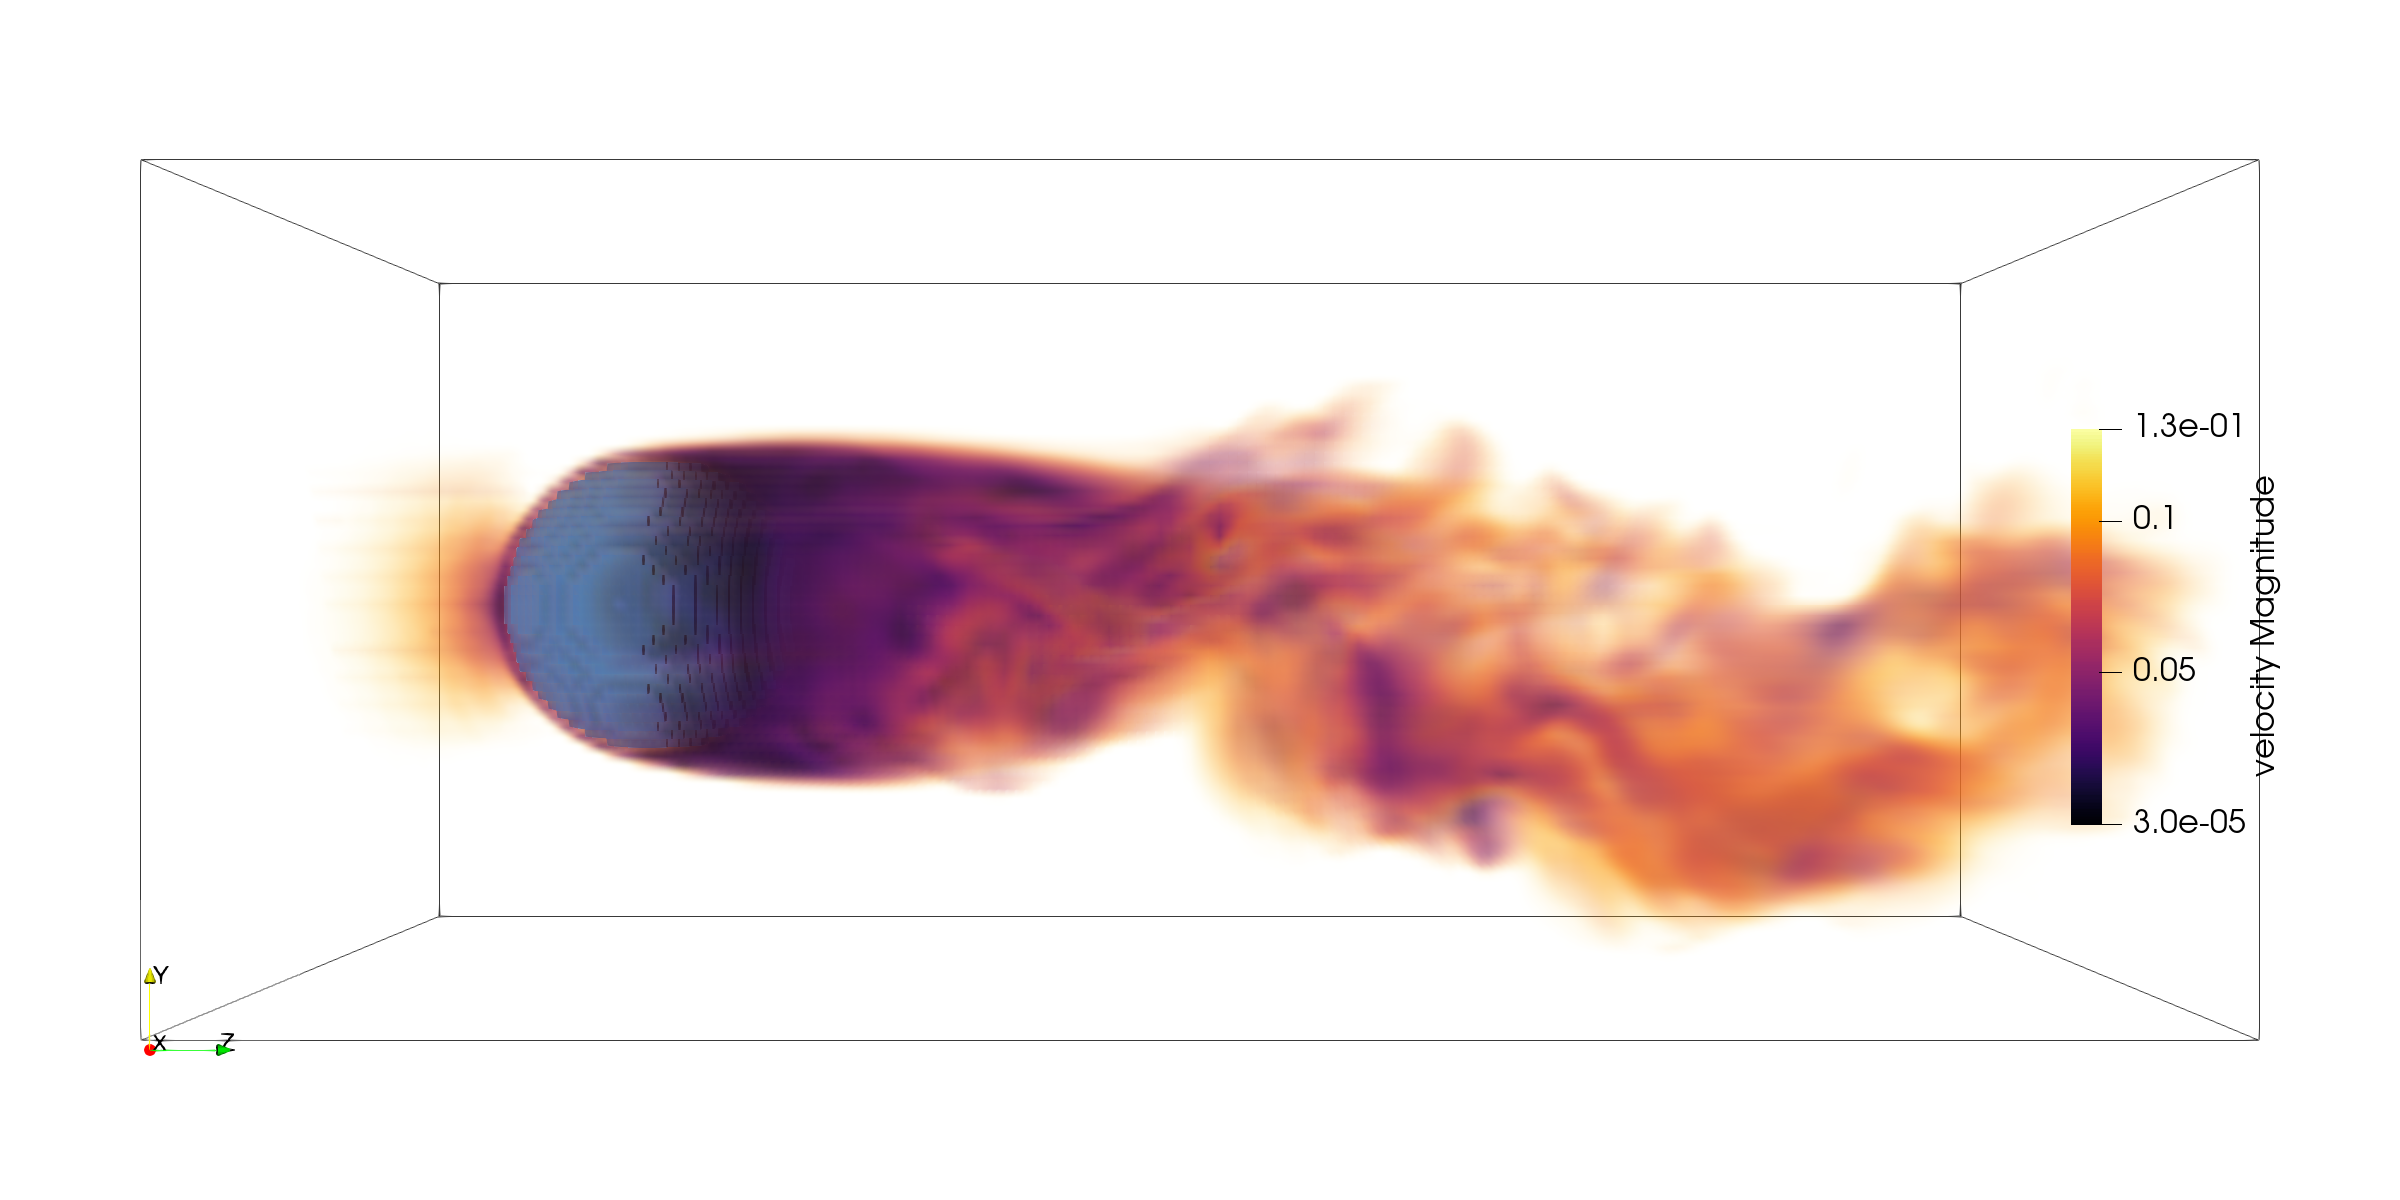
\includegraphics[width=\linewidth]{purple_render.png}
  \end{center}
\end{frame}
\placelogotrue


%%%
%%% cm_lbm slides
%%%

%% TODO: import cm_lbm slides

 % Graphicsfinal conclusion
\begin{frame}{Graphics Final Conclusion}
  \begin{outline}
    \1 How are we feeling about the paper title?
    \2 MRT Lattice Boltzmann methods?
    \2 Code generation using \lstinline{sympy}?
    \1 LBM + \lstinline{sympy}
      \2 \href{http://literatelb.org}{``A Literate Lattice Boltzmann Code''} \cite{web:literatelbm}
  \end{outline}
  \begin{center}
    \includegraphics[width=0.8\linewidth]{title_header.png}
  \end{center}
\end{frame}


%%
%% Paper Slides
%%


% Background Projects
\begin{frame}{Paper Context}
  \begin{outline}
    \1 Collaborative HPC work at German University
    \1 \href{https://www.fau.eu}{Fridrich-Alexander-Universit{\"a}t}
    \1 HPC stuff? 
  \end{outline}
\end{frame}

\placelogofalse
\begin{frame}{waLBerla}
\begin{columns}
\column{0.48\linewidth}
\begin{outline}
  \1 waLBerla framework 
  \2 Introduced in \cite{Bauer2021} (2021)
  \2 HPC-scale simulations
  \2 Stencil problems specifically
  \2 Bring your Compute Kernels
  \1 Provides:
  \2 Multi-node domain partitioning
  \2 Communication patterns 
  \2 Checkpoints
\end{outline}
\column{0.48\linewidth}
\begin{center}
  \shadowimage[width=0.8\linewidth]{juwels.png}
  \vspace{0.5cm}
  \includegraphics[width=0.8\linewidth]{walberla_partition.png}
  \vspace{0.5cm}
  \includegraphics[width=0.8\linewidth]{walberla_examples.png}
\end{center} 
\end{columns}
\blfootnote{From \href{t}{TODO}, \cite{Bauer2021}}
\end{frame}
\placelogotrue


\begin{frame}{\lstinline{pystencils}}
\begin{columns}
  \column{0.48\linewidth}
  \begin{outline}
  \1 Introduced in 2019 \cite{Bauer2019}
  \1 Stencil Compiler 
  \2 \lstinline{sympy}

  \2 Generates optimized compute Kernels
  \2 Introduced in \cite{Bauer2021} (2020)
  \end{outline}

  \column{0.48\linewidth}
  \centering
  \begin{center}
    \includegraphics[width=0.2\linewidth]{pystencils_logo.png}
  \end{center}
\end{columns}
\end{frame}

\begin{frame}{\lstinline{lbmpy}}
  \begin{columns}
  \column{0.48\linewidth}
  \begin{outline}
  \1 Python package for LBM
  \2 Introduced in \cite{Bauer2021} (2020)
  \end{outline}

  \column{0.48\linewidth}
  \centering
  \begin{center}
    \includegraphics[width=0.2\linewidth]{lbmpy_logo.png}
  \end{center}
\end{columns}
\end{frame}


% Paper intro
\placelogofalse
\begin{frame}{Introduction}
\begin{columns}
\column{0.48\linewidth}
\begin{outline}
  \1 Presenting \cite{Hennig2023} (2023)
  \1 Re-architecture of {lbmpy}
  \2 Zero-centered Storage
  \2 Central Moment (CM)
  \2 Cumulants (K)
  \2 Support more generic governing eqns
  \1 Minimizes arithmetic operations for CM and K methods
  \1 Demonstrate small relative cost compared to SRT
\end{outline}
\column{0.48\linewidth}
\begin{center}
  \shadowimage[width=0.46\linewidth]{hennig_paper.png}

  \includegraphics[width=0.28\linewidth]{frederik_hennig.jpg}
  \includegraphics[width=0.28\linewidth]{markus_holzer.jpg}

  \includegraphics[width=0.28\linewidth]{ulrich_rude.jpg}
\end{center} 
\end{columns}
\end{frame}
\placelogotrue



% Zero-centered
\begin{frame}{Zero-centered Storage}
TODO
\end{frame}


% TODO Simplication Passes 
\begin{frame}{Simplification Passes}
  \begin{columns}
  \column{0.58\linewidth}
  \begin{outline}
    \1 Conserved Quantity Rewriting
    \2 Use moments instead of $\rho, \bm{u}$
    \1 Propagation of Logarithms
    \2 Relevant for Cumulants
    \1 Common Subexpression Elimination (CSE)
    \2 Make new assignments for them
    \1 Expression Propagation
    \2 For assignments with constant RHS
    \2 Copy into use-sites
    \1 Unused Subexpression Elimination
    \2 Remove unused assignments
  \end{outline}
  \column{0.38\linewidth}
  \centering
  \begin{center}
  \begin{align*}
    \kappa_{000} &= \rho \\
    \kappa_{100} &= -F_x / 2 \\
    \kappa_{000}^{*} &= \kappa_{000} \\
    \kappa_{100}^{*} &= \kappa_{100} + F_x \\
    m^{*}_{10|0} &= \kappa^{*}_{000} \bm{u}_x + \kappa_{100}^{*}
  \end{align*}
  To
  \begin{align*}
  m^{*}_{10|0} &= \rho \bm{u}_x + F_x / 2 
  \end{align*}
\end{center}
\end{columns}
\end{frame}

\begin{frame}{Moment Transform, pt. 1}
\begin{columns}
\column{0.48\linewidth}
\begin{outline}
  \1 Transform populations to Raw Moments ($Mf$)
  \1 Use Chimera transform to compute moments    
  \2 Introduced in \cite{Geier2015}
  \1 More efficient than Matrix transform
  \1 Inverse uses trick to split populations \\
  $f^{*}_i = f^{+}_i + f^{-}_i, \ f^{*}_{\bar{i}} = f_i^{+} - f^{-}_i$
\end{outline}

\column{0.48\linewidth}

\centering
\begin{center}
\begin{align*}
  m_{xy|\gamma} &:= \sum_{z \in \{-1, 0, 1\}} f_{xyz} \cdot z^{\gamma} \\ 
  m_{x|\beta\gamma} &:= \sum_{y \in \{-1, 0, 1\}} m_{xy|\gamma} \cdot y^{\beta} \\ 
  m_{\alpha\beta\gamma} &:= \sum_{x \in \{-1, 0, 1\}} m_{x|\beta\gamma} \cdot x^{\alpha} \\ 
\end{align*}
\end{center}
\end{columns}
\end{frame}

\begin{frame}{Moment Transform, pt. 2}
\begin{columns}
\column{0.48\linewidth}
\begin{outline}
  \1 To compute central moments
  \1 First compute raw moments $m_{\alpha\beta\gamma}$
  \1 Then transform them to central moments $\kappa_{\alpha\beta\gamma}$
\end{outline}

\column{0.48\linewidth}

\centering
\begin{center}
\begin{align*}
  \kappa_{ab|\gamma} &:= 
  \sum_{c = 0}^{\gamma} \binom{\gamma}{c} (-u_z)^{\gamma - c} m_{a b c} \\
  \kappa_{a|\beta\gamma} &:= 
  \sum_{c = 0}^{\gamma} \binom{\gamma}{c} (-u_z)^{\gamma - c} m_{a b c} \\
\end{align*}
\end{center}
\end{columns}

  \begin{align*}
    \kappa_{\alpha\beta\gamma} = 
    \sum_{a, b, c = 0}^{\alpha\beta\gamma} 
    \binom{\alpha}{a} \binom{\beta}{b} \binom{\gamma}{c} 
    (-u_x)^{\alpha - a}(-u_y)^{\beta - b} (-u_z)^{\gamma - c} m_{a b c}
  \end{align*}


\end{frame}



% "Operation Count"
% rg '\+|\*|\-' cm_lbm_generated/src/shader_ops/cm_mrt.rs -o  | wc -l
\begin{frame}{Symbolic Simplification Results}
  \centering
  \begin{center}
    \includegraphics[width=0.8\linewidth]{arith_table.png}
  \end{center}
  For reference, my had \textsc{CM} implementation (slight over estimate) $220,702$ arithmetic operations.
  \blfootnote{From \cite{Hennig2023}}
\end{frame}






% Eh
% \begin{frame}
  \begin{outline}
   \1 \cite{Yu2025Filter}
  \end{outline}
\end{frame}


\begin{frame}[allowframebreaks]{References}
    \tiny
    \printbibliography
\end{frame}

\end{document}


